\documentclass[thesis.tex]{subfiles}

%%%%%%%%%%%%%%%%%%%%%%%%%%%%%%%%%%%%%%%%

\pgfplotsset{width=7cm,compat=1.8}
\definecolor{darkgreen}{RGB}{0,127,0}

\definecolor{wmle}{RGB}{0,0,0}
\definecolor{wmlei}{RGB}{230,159,0}
\definecolor{wave}{RGB}{86,180,233}
\definecolor{wboot}{RGB}{204,121,167}
\definecolor{wowa}{RGB}{0,158,115}

%%%%%%%%%%%%%%%%%%%%%%%%%%%%%%%%%%%%%%%%

%\newcommand{\smin}[1]{s_\text{min}({#1})}
\newcommand{\smin}{s_\text{min}}
\newcommand{\smax}{s_\text{max}}
\newcommand{\qhi}{\alpha_\text{hi}}
\newcommand{\qlo}{\alpha_\text{lo}}
\newcommand{\zero}{\text{\textbf{0}}}
\newcommand{\Zproj}{Z^{\textit{proj}}}
\newcommand{\Zowa}{Z^{\textit{owa}}}
\newcommand{\nowa}{n^{\textit{owa}}}
\newcommand{\Q}{\mathcal{Q}}
\newcommand{\Y}{\mathcal{Y}}
\newcommand{\X}{\mathcal{X}}
\newcommand{\matW}{\hat W}
\newcommand{\matV}{\hat V}
\newcommand{\W}{{\mathcal W}}
\newcommand{\Wowa}{{\hat \W^{\textit{owa}}}}
\newcommand{\Waff}{\mathcal{\hat A}}
\newcommand{\WaffE}{{\mathcal{\hat A}_\E}}
\newcommand{\Wave}{{\mathcal{\hat W}^{ave}}}
\newcommand{\Wtave}{{\mathcal{W}^{ave,*}}}
\newcommand{\V}{\mathcal{V}}
\newcommand{\A}{\mathcal{A}}
\newcommand{\D}{\mathcal{D}}
\newcommand{\x}{\mathbf{x}}
\newcommand{\y}{\mathbf{y}}
\newcommand{\w}{\mathbf w}
\newcommand{\vv}{\mathbf{v}}
\newcommand{\vfull}{\hat\vv^{\textit{owa,full}}}
\newcommand{\vowa}{\hat\vv^{\textit{owa}}}
\newcommand{\vstar}{\vv^{\textit{*}}}
\newcommand{\wkl}{\hat\w^{kl}}
\newcommand{\astar}{\vv^*}
\newcommand{\wowa}{\hat\w^{owa}}
\newcommand{\wowafull}{\hat\w^{\textit{owa,full}}}
\newcommand{\wowastar}{\hat\w^{\textit{owa,*}}}
\newcommand{\wave}{\hat\w^{ave}}
\newcommand{\wtave}{\E\hat\w^{ave}}
\newcommand{\waver}{\hat\w^{ave,r}}
\newcommand{\wboot}{\hat\w^{boot}}
\newcommand{\wmle}{\hat\w^{erm}}
\newcommand{\wmler}{\hat\w^{erm,r}}
\newcommand{\wstar}{{\w^{*}}}
\newcommand{\what}{{\hat\w}}
\newcommand{\wq}{\hat\w^{q}}
\newcommand{\wqstar}{\hat\w^{q^*}}
\newcommand{\dist}{\mathcal{D}}
\newcommand{\reg}{r}
\newcommand{\loss}{\ell}
\newcommand{\Loss}{\mathcal{L}^*}
\newcommand{\Lossstar}{\mathcal{L}^*}

\newcommand{\tbias}{t_{\text{\textit{bias}}}}
\newcommand{\tvar}{t_{\text{\textit{var}}}}


\newcommand{\plots}[1]{\tikz[baseline=0.6ex]\draw (0,0) rectangle (1in,1.4in);}
%\newcommand{\plots}[1]{#1}

%%%%%%%%%%%%%%%%%%%%%%%%%%%%%%%%%%%%%%%%%%%%%%%%%%%%%%%%%%%%%%%%%%%%%%%%%%%%%%%%

\begin{document}

\chapter{Merging via optimization}

%\begin{abstract}
We present the \emph{optimal weighted average} (OWA) distributed estimator for linear models. 
OWA achieves statistically optimal learning rates even on non-convex problems.
Depending on the computational model, OWA requires either only one or two rounds of communication.
%In this method, local models are first trained on each of the compute nodes;
The algorithm first trains local models on each of the compute nodes;
then a master machine merges the models using a second round of optimization. 
This second optimization uses only a small fraction of the data, 
and so has negligible computational and communication cost.
Compared with similar distributed estimators that merge locally trained models,
OWA either has stronger statistical guarantees, 
is applicable to more models,
or has a more computationally efficient merging procedure.
%\end{abstract}

%%%%%%%%%%%%%%%%%%%%%%%%%%%%%%%%%%%%%%%%

\section{INTRODUCTION}

Many datasets are too large to fit in the memory of a single machine.
To analyze them, we must partition the data onto many machines and use distributed algorithms.
Existing distributed learning algorithms fall into one of two categories:
%Existing distributed algorithms can be classified as either interactive or non-interactive depending on their communication complexity.
%In this paper we propose an algorithm that exhibits the benefits of both types.

\emph{Interactive} algorithms require many rounds of communication between machines.
Representative examples include \citet{boyd2011distributed}, \citet{li2014scaling}, \cite{ma2015adding}, and \cite{zhao2017scope}. 
These algorithms resemble standard iterative algorithms where each iteration is followed by a communication step. 
The appeal of interactive algorithms is that they enjoy the same statistical performance as standard sequential algorithms.
That is, given $m$ machines each with $n$ data points of dimension $d$, interactive algorithms have error that decays as $O(\sqrt{d/mn})$.
But, interactive algorithms have three main disadvantages.
First, these algorithms are slow when communication latency is the bottleneck.
An extreme example occurs in the \emph{federated learning} environment proposed by \cite{mcmahan2017communication}, which uses cell phones as the computational nodes. 
Second, these algorithms require special implementations.
They do not work with off-the-shelf statistics libraries provided by (for example) Python, R, and Matlab.
Third, because of the many rounds of communication, any sensitive information in the data is likely to leak between machines.

\emph{Non-interactive} algorithms require only a single round of communication.
Each machine independently solves the learning problem on a small subset of data,
then a master machine merges the solutions together.
These algorithms solve all the problems of interactive ones:
they are fast when communication is the main bottleneck;
they are easy to implement with off-the-shelf statistics packages;
and they are robust to privacy considerations.
The downside is worse statistical performance.
The popular averaging estimator has worst case performance $O(\sqrt{d/n})$ completely independent of the number of machines $m$. 
A growing body of work improves the analysis of the averaging estimator under special conditions 
(e.g.
\citet{mcdonald2009efficient},
\citet{zhang2012communication},
\citet{zhang2013divide},
and
\citet{rosenblatt2016optimality})
and develops more robust non-interactive estimators
(e.g.
\citet{zinkevich2010parallelized},
\citet{liu2014distributed},  
\citet{lee2015communication}, 
\citet{battey2015distributed},
\citet{han2016bootstrap},
and \citet{jordan2016communication}).
Existing estimators either work on only a limited class of models or have computationally intractable merge procedures.

%Non-interactive learning alg
%The popular large scale learning system Vowpal Wabbit combines both types of algorithms to achieve good real world performance.
%A non-interactive algorithm is run first to provide a good warm start to a subsequent interactive algorithm \citep{agarwal2014reliable}.

In this paper, we propose a novel non-interactive estimator called the \emph{optimal weighted average} (OWA).
%OWA requires only one round of communication,
%but the merge procedure performs a second optimization over the data. 
%The key insight of OWA is to use a second round of optimization over the data in the merge procedure.
OWA's merge procedure uses a second round of optimization over the data.
(All previous merge procedures do not depend on the data.)
This data dependent merge procedure has four advantages:
(i) OWA achieves the optimal error of $O(\sqrt{d/mn})$ in a general setting and with a simple analysis.
In particular, we do not require a convex loss function.
(ii) This second optimization uses a small number of data points projected onto a small dimensional space. 
It therefore has low computational and communication overhead.
(iii) OWA is easily implemented in a MapReduce architecture with standard packages.
Our implementation uses only a few dozen lines of Python.
(iv) OWA is robust to the regularization strength used in the first round of optimization.
In practice, this means that OWA does not require communication between nodes even in the model selection step of learning.
No previous one-round estimator has considered the cost of communication during model selection.
%In the second round of communication, the machines send only a small amount of data.
%So OWA retains the speed advantages of non-interactive estimators.
%The algorithm has two tunable parameters that let the user trade better statistical performance for worse communication complexity.
%These parameters do not require cross-validation to set correctly;
%increasing the amount of communication will always improve the statistical performance.
%Therefore, these parameters are determined by the communication constraints and not the underlying data.
%The amount of information communicated in the second round is small, however,
%so our algorithm retains the speed advantages of non-interactive algorithms.

%In the next section, we formally describe the OWA algorithm.
Section 2 formally describes our problem setting, and
Section 3 describes the OWA algorithm.
We take special care to show how OWA can be implemented with off-the-shelf optimizers.
Section 4 provides a simple proof that OWA achieves the optimal $O(\sqrt{d/mn})$ error. %under mild conditions.
Our main condition is that the single machine parameter vectors have a ``sufficiently Gaussian'' distribution.
This is a mild condition known to hold in many situations of interest.
In order to clarify the constant factors involved in our algorithm,
we also introduce a novel measure of the smoothness of a loss function.
%We also introduce a novel way to quantify the smoothness of a loss function.
Section 5 compares OWA to existing distributed algorithms.
We highlight how the analysis of existing algorithms requires more limiting assumptions than OWA's.
%and show in detail why existing non-interactive regret bounds do not apply to OWA.
Section 6 shows empirically that OWA performs well on synthetic and real world advertising data.
We demonstrate that OWA is robust to the strength of regularization,
which is one of the reasons it performs well in practice.


%\subsection{Performance Bounds}
%\label{sec:bounds}

%Performance bounds come in two flavors: statistical and information theoretic.
%On the statistical side, \citet{liu2014distributed} show that for any non-interactive distributed estimator $\what$,
%the quantity $\ltwo{\what-\wmle}{}^2$ decays as $\Omega(\gamma^2 \I^{-1}/n^2)$.
%Here $\gamma$ is the statistical curvature of the model and $\I$ is the Fisher information.
%Furthermore, they show that their KL-averaging estimator $\wkl$ matches this bound.
%One consequence of this bound is that no non-interactive learner can achieve the optimal $O(\sqrt{d/mn})$ error on models with nonzero statistical curvature.
%The vast majority of models used in practice have nonzero curvature.
%The only models with zero curvature are full exponential families.
%OWA is able to ``break'' this bound and achieve optimal error rate because of its semi-interactive setting.
%A crucial assumption of Liu and Ihler's analysis is that the merge function not depend on the data.

%\citet{shamir2014fundamental}, \citet{zhang2013information}, and \citet{garg2014communication} all provide information theoretic lower bounds on the sample complexity of non-interactive learning problems.
%As above, however, their results are not applicable in our semi-interactive setting.
%\citet{braverman2015communication} provide a bound that applies in all distributed settings.
%In particular, they show that the minimax optimal error rate for least squares regression requires $\Omega(m\cdot\min\{n,d\})$ bits of communication.
%Surprisingly, this dependence on $d$ remains even when $\wstar$ is highly sparse. 
%%This dependence on $d$ remains even when the number of nonzero entries of $\wstar$ is much less than $d$.
%This bound essentially matches the communication complexity of Algorithm 1. %where we have assumed the master already has access to $\Zowa$.
%There is one information theoretic lower bound that does apply to us.
%Let the true parameter vector $\wstar$ be $k$-sparse.
%That is, $\lzero{\wstar} \le k$.
%%Then \cite{zhang2013information} showed that at least $\Omega(mk/\log m)$ bits of communication are required in the non-interactive setting,
%%and \cite{garg2014communication} improved this lower bound to $\Omega(mk)$.
%Surprisingly, \citet{braverman2015communication} show that the minimax optimal error rate for least squares regression requires $\Omega(m\cdot\min\{n,d\})$ bits of communication (independent of $k$) independent of the setting.
%This is important because sparsity does not reduce the amount of communication required, and this bound does apply in our setting.
%Recall that the communication cost of OWA is $O(dm^2+m^2n/d)$, which is looser than the lower bound.
%\section{THE OWA ALGORITHM}
%
%This section first formally introduces the problem of communication efficient distributed estimation,
%then describes our proposed OWA distributed estimator.
%
%\subsection{Problem Setting}

%%%%%%%%%%%%%%%%%%%%%%%%%%%%%%%%%%%%%%%%%%%%%%%%%%%%%%%%%%%%%%%%%%%%%%%%%%%%%%%%

\vspace{-0.1in}
\section{PROBLEM SETTING}

\vspace{-0.05in}
Let $\Y\subseteq\mathbb{R}$ be the space of response variables,
$X\subseteq\mathbb{R}^d$ be the space of covariates,
and $\W\subseteq\mathbb{R}^d$ be the parameter space.
%A model is specified by a loss function $f:\Y\times\mathbb R\to\mathbb R$.
We assume a linear model where the loss of data point $(\x,y)\in\X\times\Y$ given the parameter $\w\in\W$ is denoted by $\loss(y,\trans\x\w)$.
We define the true loss of parameter $\w$ to be $\Lossstar(\w) = \E\loss(y;\trans\x\w)$, 
and the optimal parameter vector $\wstar=\argmin_{\w\in\W}\Lossstar(\w)$.
We do not require that the model be correctly specified,
nor do we require that $\loss$ be convex with respect to $\w$.
Let $Z\subset\X\times\Y$ be a dataset of $mn$ i.i.d.\ observations.
Finally, let $\reg : \W \to \mathbb{R}$ be a regularization function (typically the L1 or L2 norm)
and $\lambda\in\mathbb{R}$ be the regularization strength.
Then the regularized empirical risk minimizer (ERM) is
\begin{equation}
\label{eq:wmle}
%\wmle=\argmax_\w \sum_{i=1}^{mn} g(y_i-\trans\x_i\w)
\wmle=\argmax_{\w\in\W} \sum_{(\x,y)\in Z} \loss(y,\trans\x\w)
+ \lambda \reg(\w)
.
\end{equation}
%In the remainder of this paper, it should be understood that all ERMs are regularized.
%
Assume that the dataset $Z$ has been partitioned onto $m$ machines so that each machine $i$ has dataset $Z_i$ of size $n$, and all the $Z_i$ are disjoint.
Then each machine calculates the local ERM
\begin{equation}
\label{eq:wmlei}
\wmle_i = \argmax_{\w\in\W} \sum_{(\x,y) \in Z_i} \loss(y,\trans\x\w)
+ \lambda \reg(\w)
.
\end{equation}
Solving for $\wmle_i$ requires no communication with other machines.
Our goal is to merge the $\wmle_i$s into a single improved estimate.
A baseline merging procedure is the averaging estimator:
\begin{equation}
\wave = \frac{1}{m}\sum_{i=1}^m \wmle_i
.
\end{equation}
This estimator is well studied.
%, and in Section \ref{sec:relwork} we compare this previous work to our own.
Recall that the quality of an estimator $\what$ can be measured by the estimation error $\ltwo{\what-\wstar}$. 
We can use the triangle inequality to decompose this error as
\begin{equation}
%\ltwo{\wave-\wstar} \le \ltwo{\wave-\E\wave}+ \ltwo{\E\wave - \wstar } .
\ltwo{\what-\wstar} \le \ltwo{\what-\E\what}+ \ltwo{\E\what - \wstar } .
\end{equation}
We refer to $\ltwo{\what-\E\what}$ as the variance of the estimator and $\ltwo{\E\what-\what}$ as the bias.
%$\ltwo{\wstar-\wave}$ can be decomposed into bias $\ltwo{\wstar - \E\wave}$ and variance $\ltwo{\E\wave-\wave}$ components.
\citet{mcdonald2009efficient} show that the $\wave$ estimator has lower variance than the estimator $\wmle_i$ trained on a single machine, but the same bias.
\citet{zhang2012communication} extend this analysis to show that if $\wmle_i$ is a ``nearly unbiased estimator'' then the mean squared error (MSE) $\E\ltwo{\wstar-\wave}{}^2$ decays as $O((mn)^{-1} + n^{-2})$.
%Our goal is to design an estimator that reduces both variance and bias.
Both results require $\loss$ to be convex in addition to other technical assumptions.
Our goal is to design a merging procedure that has good error bounds in a more general setting.

%%%%%%%%%%%%%%%%%%%%%%%%%%%%%%%%%%%%%%%%%%%%%%%%%%%%%%%%%%%%%%%%%%%%%%%%%%%%%%%%%%%%%%%%%%

\vspace{-0.1in}
\section{THE OWA ESTIMATOR}

\vspace{-0.05in}
%We propose a modification to the averaging estimator called the \emph{optimal weighted average} (OWA). 
The \emph{optimal weighted average} (OWA) estimator uses a second round of optimization to calculate the optimal linear combination of the $\wmle_i$s.
%Using these optimal weights, we reduce bias at a rate of $O(\sqrt{1-m/d})$.
This second optimization occurs over a small fraction of the dataset,
so its computational and communication cost is negligible.

\subsection{Warmup: The Full OWA}

To motivate the OWA estimator,
we first present a less efficient estimator that uses the full dataset for the second round of optimization.
%The idea of our proposed solution is to find the best linear combination of the $\wmle_i$s using a second round of optimization.
Define the matrix $\matW : \mathbb{R}^{d\times m}$ to have its $i$th column equal to $\wmle_i$. 
Now consider the estimator
\begin{equation}
\wowafull = \matW \vfull
,
%\end{equation}
\text{~~~~~where~~~~~}
%\begin{equation}
\label{eq:vfull}
\vfull = \argmax_{\vv\in\mathbb R^m} \sum _{(\x,y)\in Z} \loss\left(y,\trans\x \matW \vv \right)
+
\lambda \reg(\matW\vv)
.
\end{equation}
Notice that $\wowafull$ is just the empirical risk minimizer when the parameter space $\W$ is restricted to the subspace $\Wowa=\vecspan\{\wmle_i\}_{i=1}^m$.
In other words, the $\vfull$ vector contains the optimal weights to apply to each $\wmle_i$ when averaging.
Figure \ref{fig:contour} shows graphically that no other estimator in $\Wowa$ can have lower regularized empirical loss than $\wowafull$.

\begin{wrapfigure}{R}{0.5\textwidth}
\vspace{-0.25in}
\hspace{-0.1in}
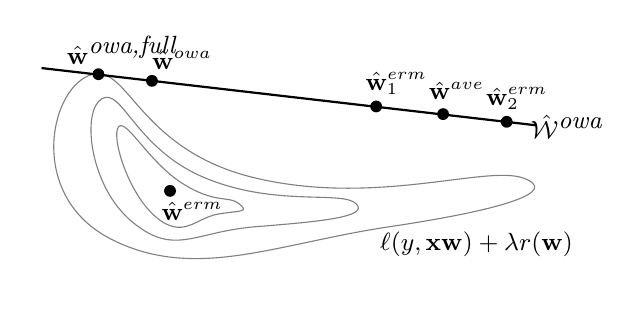
\begin{tikzpicture}
    [
    dot/.style = {minimum width=0.15cm,inner sep=0pt,line width=0pt,fill,circle,black,font=\small}
    , xscale=0.85
    , yscale=0.65
    ]
\small
\draw[gray] plot [smooth cycle,tension=1] coordinates {(-0.5,-0.75) (-1.05,1) (-0.1,-0.1) (0.75,-0.5) (0.45,-0.7) };
\draw[gray] plot [smooth cycle,tension=1] coordinates {(-0.85,-0.85) (-1.3,1.55) (0.25,0) (2.5,-0.5) (1,-0.95)};
\draw[gray] plot [smooth cycle,tension=1] coordinates {(-1.15,-1.2) (-1.5,2) (1,0) (5,0) (3,-0.95)};

\draw[thick] (-2.2,2.15) -- (5.2,1.03);

\node[dot] (wstar) at (-0.28,-0.25) {};
\node at (0.05,-0.65) {$\wmle$};

%\node[dot] (wstarproj) at (0.1,1.8) {};
%\draw (wstar) -- (wstarproj);
%\draw (0.07,1.65) -- (0.23,1.62) -- (0.26,1.78);

%\node[dot] (wavestar) at (4,0.5) {};
%\node                 at (4.5,0.3) {$\E\wave$};
\node[dot] (wave) at (3.8,1.25) {};
\node at (4.0,1.7) {$\wave$};
\node[dot] (wave) at (2.80,1.40) {};
\node at (3.1,1.85) {$\wmle_1$};
\node[dot] (wave) at (4.75,1.10) {};
\node at (4.9,1.55) {$\wmle_2$};
%\node[dot] (wave) at (3.8,1.25) {};

\node[dot] at (-1.35,2.03) {};
\node at (-1.0,2.5) {$\wowafull$};

\node[dot] at (-0.55,1.9) {};
\node at (-0.1,2.3) {$\wowa$};

\node at (4.3,-1.3) {$\loss(y,\trans\x\w)+\lambda \reg(\w)$};
\node at (5.65,1.0) {$\Wowa$};
\end{tikzpicture}
\vspace{-0.25in}
\caption{
    $\wowafull$ is the estimator with best loss in $\Wowa$,
    and $\wowa$ is close with high probability.
    \vspace{-0.15in}
    %OWA performs a second optimization to find the best parameter vector in $\Wowa$.
    %Since $\Wowa$ has low dimension, this optimization needs relatively little data to ensure that with high probability $\wowa$ has lower empirical loss than $\wave$.
}
\label{fig:contour}
\end{wrapfigure}

\subsection{The OWA Estimator}

Calculating the weights $\vfull$ directly is infeasible because it requires access to the full dataset.
Fortunately, we do not need to consider all the data points for an accurate estimator.
In a linear model, the number of data points needed is proportional to the dimensionality of the underlying space.
The parameter space $\Wowa$ is $m$-dimensional, so we need only $O(m)$ samples.
In general, $m <\!\!< n \approx O(d)$, so this second optimization requires only a tiny fraction of the original data.
%The dimensionality of the data is typically much larger than the number of machines (i.e. $m <\!\!< d)$.
This intuition motivates the OWA estimator.
Let $\Zowa_i\subset Z_i$ be a set of $\nowa$ data points uniformly sampled from $Z_i$ without replacement,
and let $\Zowa$ be the union of the $\Zowa_i$s.
Then the OWA estimator is defined as
\begin{equation}
\label{eq:wowa}
\wowa = \matW \vowa,
%\end{equation}
\text{~~~~~where~~~~~}
%\begin{equation}
%\label{eq:ahat}
\vowa = \argmax_{\vv\in\mathbb R^m} \sum _{(\x,y)\in \Zowa} \loss\left(y,\trans\x \matW \vv \right)
+ \lambda \reg(\matW\vv)
.
\end{equation}

%\begin{figure}
%\begin{minipage}{\textwidth}

%\begin{tabular}{lr}
\begin{wrapfigure}{R}{0.475\textwidth}
\vspace{-0.30in}
\begin{minipage}{0.475\textwidth}
\begin{algorithm}[H]
\caption{Calculating $\wowa$ in one round}
\label{alg:distributed}
\begin{algorithmic}
    \State \hspace{-0.1in}Preconditions: 
    \State \hspace{-0.1in}~~~~~each machine $i$ already has dataset $Z_i$
    \State \hspace{-0.1in}~~~~~the master machine additionally has $\Zowa$
    \State \hspace{-0.1in}Round 1, each machine $i$ independently:
    \State \hspace{-0.1in}~~~~~calculates $\wmle_i$ using \eqref{eq:wmlei}
    \State \hspace{-0.1in}~~~~~transmits $\wmle_i$ to the master
    \State \hspace{-0.1in}The master calculates $\wowa$ using \eqref{eq:wowa} %and \eqref{eq:ahat}
    \State \hspace{-0.1in}~~~~~(optionally) master uses approximation \eqref{eq:approxreg}
\end{algorithmic}
\label{fig:alg1}
\end{algorithm}
%\end{minipage}
%\end{wrapfigure}
%&
%\begin{wrapfigure}{R}{0.475\textwidth}
%\begin{minipage}{0.475\textwidth}
\vspace{-0.25in}
\begin{algorithm}[H]
\caption{Calculating $\wowa$ in two rounds}
\label{alg:distributed}
\begin{algorithmic}
    \State \hspace{-0.1in}Preconditions:
    \State \hspace{-0.1in}~~~~~each machine $i$ already has dataset $Z_i$
    \State \hspace{-0.1in}Round 1, each machine $i$ independently:
    \State \hspace{-0.1in}~~~~~calculates $\wmle_i$ using \eqref{eq:wmlei}
    \State \hspace{-0.1in}~~~~~broadcasts $\wmle_i$ to all other machines
    \State \hspace{-0.1in}Round 2, each machine $i$ independently:
    \State \hspace{-0.1in}~~~~~constructs $\matW=(\wmle_1,...,\wmle_m)$
    \State \hspace{-0.1in}~~~~~samples a dataset $\Zowa_i\subset Z_i$ of size $\nowa$
    \State \hspace{-0.1in}~~~~~calcs $\Zproj_i=\{(\trans\x\matW,y) : (\x,y)\in\Zowa\}$
    \State \hspace{-0.1in}~~~~~sends $\Zproj_i$ to a master machine
    \State \hspace{-0.1in}The master calculates $\wowa$ using \eqref{eq:wowa} %and \eqref{eq:ahat}
    \State \hspace{-0.1in}~~~~~(optionally) master uses approximation \eqref{eq:approxreg}
\end{algorithmic}
\label{fig:alg2}
\end{algorithm}
\end{minipage}
\vspace{-0.20in}
\end{wrapfigure}
%\end{tabular}
%\end{minipage}
%\end{figure}

We present two algorithms for calculating $\wowa$.
Algorithm \ref{fig:alg1} uses only a single round of communication, 
but requires that a predesignated master machine already have a copy of the $\Zowa$ dataset.
Each machine calculates $\wmle_i$ independently,
then transfers the result to the master.
The master then has all the information needed to solve \eqref{eq:wowa}. 
A total of $O(dm)$ bits are transfered to the server.
(The parameter vector has $d$ dimensions and there are $m$ machines.)
The averaging estimator transfers the same information,
and so has the same $O(dm)$ communication complexity.
The only difference between the two algorithms is the way the master machine merges the local estimates.

If the master machine does not already have a copy of $\Zowa$,
then we must transfer a copy to the master. 
Algorithm \ref{fig:alg2} is a two round version of OWA that exploits the structure of the $\wowa$ estimator to transmit this data efficiently.
In the first round, each machine calculates $\wmle_i$ independently.
The result is then broadcast to every other machine, instead of just the master.
A total of $O(dm^2)$ bits are transmitted in this round.
(The parameter vector has $d$ dimensions,
there are $m$ machines,
and each machine transmits to each other machine.)
In the second round, each machine projects its local dataset $\Zowa_i$ onto the space $\Wowa$.
These projected data points are then transmitted to the master.
A total of $O(m^2\nowa)$ bits are transmitted.
(The projected data points each have dimension $m$, 
there are $m$ machines,
and there are $\nowa$ data points per machine.)
%The master machine now has all of the information to complete the optimization.
The analysis in Lemma 2 (see Section \ref{sec:anal}) suggests that $\nowa$ should be set to $O(mn/d)$.
So the total data transmitted in both rounds is $O(dm^2 + m^3n/d)$. 

%The communication complexity of Algorithm 1 is asymptotically worse than the averaging estimator, 
%which transmits only $O(dm)$ bits.
%But we claim this is not a problem for two reasons.
%First, this worse dependence on $m$ is not significant in practice because $m$ is much smaller than $n$ and $d$.
%We show in our experiments that when the problem is large enough to take a full day to solve for the $\wmle_i$s on the first round, the second round takes only several minutes.
%Second, with a slight modification to the problem setting, we can reduce the communication complexity to match the $O(dm)$ bound of the averaging estimator.
%In the original problem setting, we assume that the data points have already been communicated to the machines. 
%In particular, the $O(dm)$
%
%so whenever $d>m^2$ and $d>mn/d$, OWA has the same asymptotic communication complexity as averaging.
%When $d<m\nowa$, this is the same order of bits as the averaging estimator.

\subsection{Implementing OWA with Existing Optimizers}
\label{sec:lambda2}

Equations \ref{eq:vfull} and \ref{eq:wowa} cannot be solved directly using off-the-shelf optimizers because existing optimizers do not support the non-standard regularization term $\reg(\matW\vv)$.
%This regularization is in principle no more difficult to optimize than the term $\reg(\w)$ from Equation $\ref{eq:wmle}$;
%it is simply not implemented.
In practice, it is sufficient to approximate this term by L2 regularization directly on the $\vv$ vector:
\begin{equation}
\lambda \reg(\matW\vv) \approx \lambda_2 \ltwo{\vv}^2
,
\label{eq:approxreg}
\end{equation}
where $\lambda_2$ is a new hyperparameter.
We provide two justifications for this approximation:

\vspace{-0.05in}
\begin{enumerate}[leftmargin=0.15in]
\item
When we want the parameter vector $\w$ to be sparse 
(and so the regularizer $\reg$ is the L1 norm), 
we have no reason to believe that the $\vv$ vector should be sparse.
The desired sparsity is induced by the regularization when solving for $\wmle_i$s and maintained in any linear combination of the $\wmle_i$s.
\item
As the size of the dataset increases, the strength of the regularizer decreases.
In this second optimization, the dimensionality of the problem is small,
so it is easy to add more data to make the influence of the regularization negligible.
\end{enumerate}

\vspace{-0.05in}
The new $\lambda_2$ regularization parameter should be set by cross validation.
This will be a fast procedure, however, because there are only $m\nowa <\!\!< mn$ data points to optimize over,
they have dimensionality $m<\!\!<d$,
and the L2 regularized problem is much easier to solve than the L1 problem.
Furthermore, this cross validation can be computed locally on the master machine without any communication.
The experiments in Section \ref{sec:exp} provide an example where the first round of optimization to compute the $\wmle_i$s takes about a day, but the second round of optimization (including cross validation over $\lambda_2$) takes only several minutes.
%With this minor modification, our distributed estimator can be implemented using any existing optimizer.
%Our experimental results in Section \ref{sec:exp} use this modified version of $\hat\vv$.

%%%%%%%%%%%%%%%%%%%%%%%%%%%%%%%%%%%%%%%%%%%%%%%%%%%%%%%%%%%%%%%%%%%%%%%%%%%%%%%%

\section{ANALYSIS}
\label{sec:anal}

In this section, we outline the argument that OWA's generalization error $\Lossstar(\wowa)-\Lossstar(\wstar)$ and estimation error $\ltwo{\wowa-\wstar}$ both decay as $O(\sqrt{d/mn})$.
Full proofs of all theorems can be found in the supplemental material.
%The proof is broken into two steps.
%First we show that $\Wowa$ is a good subspace to optimize over in the sense that the distance between $\Wowa$ and $\wstar$ is small.
%Then we show that $\wowa$ is a good parameter to choose within $\Wowa$.
%
Our analysis depends on the single machine estimators obeying the following mild condition.

%\newtheorem*{sgt}{The Sub-Gaussian Tail (SGT) Condition}
%\begin{sgt}
\begin{definition}
We say that an estimator $\what$ that has been trained on $n$ data points of dimension $d$ satisifies the \emph{sub-gaussian tail (SGT) condition} if,
%Let $\what$ be a linear estimator trained on $n$ data points of dimension $d$.
%Let $t>0$.
for all $t>0$,
with probability at least $1-\exp(-t)$,
$\ltwo{\what-\wstar} \le O( \sqrt{dt/n} ).$
%\begin{equation}
%%\ltwo{\wstar-\what} \le O\left( \sqrt\frac {dt} {n} \right)
%\ltwo{\wstar-\what} \le O\left( \sqrt{dt/n} \right)
%.
%\label{eq:sgt}
%\end{equation}
%\end{sgt}
\end{definition}

%Sub-Gaussian distributions have recently become an important tool in the analysis of high dimensional statistics.
%\cite{vershynin2010introduction} provides an accessible tutorial of these results.

The SGT condition is a high-level condition that is well established in the statistical literature.
All generalized linear models (such as logistic regression and ordinary least squares regression) satisfy the SGT condition,
and many less standard models (such as linear models with a sigmoid loss) also satisfy the condition. 
There are many ways to prove that an estimator satisfies the SGT condition.
In the asymptotic regime when $n\to\infty$,
very strong results of this form have been known since the 1960s.
Chapter 7 of \citet{lehmann1999elements} provides an elementary introduction to this work.
Lehman requires only that $\loss$ be three times differentiable, that the data points be i.i.d., and that $\wstar$ be identifiable.
More recent results establish the SGT condition in the non-asymptotic regime $n<\infty$.
%The simplest results place distributional assumptions on the data.
%For example, \citet{negahban2009unified} considers the case when the data points are sub-Gaussian, the likelihood satisfies a ``restricted strong convexity condition,'' and the regularizer is decomposable.
%Their resulting theorems are actually much stronger than the SGT condition:
%They prove that the dependence on the dimension $d$ in Equation \ref{eq:sgt} can be replaced by the number of non-zero elements in the optimal parameter vector $\wstar$.
%For sparse models, this is a major improvement.
%%\citet{sivakumar2015beyond} provides similar bounds when the data are only sub-exponential (which is more general than sub-Gaussian).
The strongest non-asymptotic results known to the authors are due to \citet{spokoiny2012parametricestimation}.
%Spokoiny does not place any distributional assumption on the data,
%captures sparsity information through dependence on the Fisher information,
%and does not even require the data to be i.i.d.
Spokoiny's only assumption is that the empirical loss admit a local approximation via the ``bracketing device,''
which is a generalization of the Taylor expansion.
The full explanation of the bracketing device is rather technical,
so we do not present it here.
Instead, we highlight that Spokoiny's results do not require a convex loss or even that the data be i.i.d. 

The first lemma is an easy consequence of the SGT condition for the $\wmle_i$s.
It formalizes the key idea that $\Wowa$ is a good subspace to optimize over because it contains a point close to the true parameter vector.
%\clearpage

\begin{lemma}
\label{lemma:wwstar}
Assume the $\wmle_i$s satisfy the SGT condition.
Let $\proj{\Wowa}\wstar$ denote the vector in $\Wowa$ with minimum distance to $\wstar$.
%That is, $\proj{\Wowa}\wstar$ is the vector minimizing \eqref{eq:wwstar}.
Let $t>0$. 
Then with probability at least $1-\exp(-t)$,
\begin{equation}
\label{eq:wwstar}
\ltwo{\proj{\Wowa}\wstar-\wstar} \le O(\sqrt{dt/mn})
%\min_{\w\in\Wowa}\ltwo{\w-\wstar} \le O(\sqrt{dt/mn})
%\min_{\w\in\Wowa}\ltwo{\w-\wstar} \le \sigma\sqrt{\frac{v_{t/m}}{n}}
%\prob{\min_{\w\in\Wowa}\ltwo{\w-\wstar} \ge \sqrt{\frac{v_t}{n}} } \le \exp(-tm)
.
\end{equation}
\end{lemma}

Our next lemma shows that $\wowa$ is a good approximation of $\wowafull$ as long as $\nowa=mn/d$. 
In linear models, the number of dimensions used typically grows proportionally to the number of data points, so this lemma formalizes the intuition that relatively little data is needed in the second optimization.
%Throughout this section, we will assume that the $\wmle_i$s, $\vowa$, and $\vfull$ estimators all satisfy the SGT condition.
In this lemma, we require that both $\vfull$ and $\vowa$ satisfy the SGT condition.
Recall from Equations \ref{eq:vfull} and \ref{eq:wowa} that both estimators are trained on a projected data set with dimension $\min(m,d)$.
So the SGT conditions for $\vfull$ and $\vowa$ state that with probability at least $1-\exp(-t)$,
\vspace{-0.15in}
\begin{equation}
    \ltwo{\vfull-\vstar} \le O(\min(m,d)t/mn),
    \text{~~~~~and~~~~~}
    \ltwo{\vowa-\vstar} \le O(\min(m,d)t/m\nowa),
\end{equation}
where $\vstar$ is the parameter vector in $\Wowa$ that minimizes $\Lossstar$.
(Note that in general, $\vstar\ne\proj{\Wowa}\wstar$).
The results of \citet{spokoiny2012parametricestimation} can be used to show that $\vfull$ and $\vowa$ satisfy the SGT condition.

%The main idea of our analysis is to show that $\Wowa$ is a good subspace to optimize over.
%This idea is captured in the following lemma.


\begin{lemma}
    \label{lemma:wowafullwowa}
Assume that $\vfull$ and $\vowa$ satisfy the SGT condition.
Let $\nowa=mn/d$.
Let $t>0$.
Then with probability at least $1-\exp(-t)$, $\ltwo{\wowafull-\wowa}\le O(dt/mn)$.
\end{lemma}

In order to connect the results of Lemmas 1 and 2 to the generalization error of our estimator,
we need to introduce a smoothness condition on the true loss function $\Lossstar$.
\begin{definition}
    %We call the loss function $\Lossstar$ \emph{$\beta$-Lipschitz} if for all $\w_1$ and $\w_2$,
    %we have that $|\Lossstar(\w_1)-\Lossstar(\w_2)|\le\beta\ltwo{\w_1-\w_2}$.
    We say that $\Lossstar$ is \emph{$\beta$-Lipschitz} continuous if for all $\w_1$ and $\w_2$,
    \begin{equation}
    |\Lossstar(\w_1)-\Lossstar(\w_2)|\le\beta\ltwo{\w_1-\w_2}.
    \end{equation}
    %We call the true loss function $\Lossstar$ \emph{($\rho,\wstar)$-locally $\beta$-Lipschitz} if
    %for all $\w$ satisfying $\ltwo{\w-\wstar}\le\rho$, we have that
    %$\Lossstar(\w)-\Lossstar(\wstar) \le \beta\ltwo{\w-\wstar}$.
    %We call the loss function \emph{locally $\beta$-Lipschitz} if
%for all $\w$ satisfying $\ltwo{\w-\wstar}\le\ltwo{\proj{\Wowa}\wstar-\wstar}$, $|\Lossstar(\w_1)-\Lossstar(\w_2)|\le\beta\ltwo{\w_1-\w_2}$.
%$\Lossstar(\proj{\Wowa}\wstar)-\Lossstar(\wstar) \le \beta\ltwo{\proj{\Wowa}\wstar-\wstar}$.
%$\Lossstar(\proj{\Wowa}\wstar)-\Lossstar(\wstar) \le \beta\ltwo{\proj{\Wowa}\wstar-\wstar}$.
\end{definition}
%We use Lipschitz continuity here because it is a standard, well understood tool.
%Many models have a locally $\beta$-Lipschitz loss.
%It is clear that every globally $\beta$-Lipschitz function is locally $\beta$-Lipschitz with the same constant.
%For example, logistic regression is locally Lipschitz for this reason.
%But many functions that are not globally Lipschitz are locally Lipschitz.
%In particular, every continuous function will be locally $\beta$-Lipschitz.
%Furthermore, if $\Lossstar$ is differentiable, then in the limit as $n\to\infty$, $\Lossstar$ is 0-locally Lipschitz. 
%Models with the square loss or sigmoid loss are therefore all locally Lipschitz with $\beta\to0$ as $n\to0$.
%so in the limit as $n\to\infty$, $\Lossstar(\proj{\Wowa}\wstar)-\Lossstar(\wstar)\to0$ and $\beta\to0$.
We can now present our first main result.
\begin{theorem}
Assume the $\wmle_i$s, $\vfull$, and $\vowa$ all satisfy the SGT condition.
Further assume that $\Lossstar$ is $\beta$-Lipschitz.
Let $\nowa=mn/d$.
%Further assume that $\Lossstar$ is $\beta$-Lipschitz 
%(i.e. for all $\w_1$ and $\w_2$, $|\Lossstar(\w_1)-\Lossstar(\w_2)|\le\beta\ltwo{\w_1-\w_2}$).
Let $t>0$.
%\begin{enumerate}
    %\item 
%If $\Lossstar$ is $\beta$-Lipschitz, 
Then with probability at least $1-\exp(-t)$,
\begin{equation}
    %|\Lossstar(\wowafull)-\Lossstar(\wstar)|
    %\le O(\beta\sqrt{dt/mn}),
    %\text{~~~~~and~~~~~}
    \Lossstar(\wowa)-\Lossstar(\wstar)
    \le O(\beta\sqrt{dt/mn}).
\end{equation}
%\item 
%If instead $\Lossstar$ is $\alpha$-strongly convex, then with probability at least $1-\exp(-t)$,
%\begin{equation}
    %%|\Lossstar(\wowafull)-\Lossstar(\wstar)|
    %%\le O(\sqrt{\alpha dt/mn}),
    %%\text{~~~~~and~~~~~}
    %|\Lossstar(\wowa)-\Lossstar(\wstar)|
    %\le O(\sqrt{\alpha dt/mn}).
%\end{equation}
%\end{enumerate}
\end{theorem}
The use of Lipschitz continuity in Theorem 1 sacrifices generality for interpretability.
While many losses are $\beta$-Lipschitz (e.g. log loss, hinge loss, and sigmoid loss),
many other losses are not (e.g. squared loss and exp loss).
Therefore Theorem 1 is not as general as it could be.
To improve generality of our next result, we introduce the following novel smoothness condition.

%Next, we introduce a smoothness condition that will connect the $\w$ minimizing \eqref{eq:wwstar} to $\wowafull$.
%
%\newtheorem*{hess}{The Hessian Condition}
%\begin{hess}
%For any vector $\w$ satisfying $\ltwo{\w}\le\ltwo{\wstar-\wowafull}$, we have that
%\begin{equation}
%\label{eq:hessiancondition}
%\qlo\ltwo{\w-\wstar}^2 \le \Loss(\w) - \Loss(\wstar) \le \qhi\ltwo{\w-\wstar}^2
%\end{equation}
%where $\Loss(\w) = \sum_{(\x,y)\in Z}\loss(y;\trans\x\w)+\lambda\reg(\w)$.
%\end{hess}
%
%This condition is somewhat easier to understand in the asymptotic regime as $n\to\infty$.
%In this regime, we have that $\ltwo{\wstar-\wowafull}\to0$,
%so \eqref{eq:hessiancondition} is equivalent to requiring that the condition number of the Hessian $\nabla^2\Loss(\wstar)$ be $\qhi/\qlo$.
%
%Our next theorem applies the Hessian Condition to Lemma \ref{lemma:wwstar} to the error of $\wowafull$.
%
%We are now ready to bound the error of $\wowafull$.

%Our technique for bounding the estimation error is similar to the technique for bounding the generalization error.
%In order to bound the estimation error, we introduce another smoothness condition.
%Whereas the $\beta$-Lipschitz condition above is widely used in machine learning,
%Before we used a global smoothness condition on the true loss $\Lossstar$;
%now we will use a local smoothness condition on the empirical loss $\Loss(\w) = \sum_{(\x,y)\in Z}\loss(y;\trans\x\w)+\lambda\reg(\w)$.
\begin{definition}
    %Let $R$ be a subset of $\W$ containing $\wstar$.
    Let $R\subseteq\W$.
    We call the true loss function $\Lossstar$ \emph{locally quadratically bracketed in $R$} (LQB-$R$) if for all points $\w\in R$,
\begin{equation}
    \label{eq:lqb}
\qlo\ltwo{\w-\wstar}^2 \le \Loss(\w) - \Loss(\wstar) \le \qhi\ltwo{\w-\wstar}^2
.
\end{equation}
%where 
%for all $\w$ satisfying $\ltwo{\w-\wstar}\le\ltwo{\wowafull-\wstar}$, $|\Lossstar(\w_1)-\Lossstar(\w_2)|\le\beta\ltwo{\w_1-\w_2}$.
\end{definition}
%Unlike the $\beta$-Lipschitz condition, the LQB condition is not widely used in machine learning.
%To understand the LQB-$R$ condition, first consider the case when $R=\W$.
%The leftmost inequality in \eqref{eq:lqb} states that $\Lossstar$ must grow within the set $R$.
The LQB-$R$ condition is quite general.
The leftmost inequality in \eqref{eq:lqb} is related to (but more general than) the more familiar notion of $\qlo$-strong convexity.
(We say $\Lossstar$ is $\qlo$-strongly convex if $\nabla^2\Lossstar(\w) \ge \qlo I$ for all $\w$.)
Inequality \eqref{eq:lqb}, however, requires only that $\nabla^2\Lossstar(\w) \ge \qlo I$ at the minimum point $\w=\wstar$.
The function may (for example) have local maxima elsewhere.
When $R$ has finite radius (i.e. $\ltwo{\w_1-\w_2}$ is finite for all $\w_1,\w_2\in R$),
then all continuous functions with a unique global minimum will satisfy the leftmost inequality for some value of $\qlo$.
%In particular, even non-convex functions will satisfy the inequality.
The rightmost inequality of \eqref{eq:lqb} states that $\Lossstar$ must not grow too quickly within $R$.
If $R$ has finite radius, and there is an open ball around $\wstar$ that does not intersect $R$,
then any continuous function satisfies the rightmost inequality for some $\qhi$.
%The LQB-R condition, however, requires only that $\nabla^2\Lossstar(\wstar) \ge \qlo I$.
In particular, models using the log loss, hinge loss, sigmoid loss, squared loss, and exp loss all satisfy the LQB-$R$ condition for any finite set $R$. 
%Our most general result is then:

\begin{theorem}
\label{theorem:wowafull}
Assume the $\wmle_i$s, $\vfull$, and $\vowa$ all satisfy the SGT condition.
%Further assume that $\Loss$ is locally quadratically bracketed in $R=\{\wowa,\wowafull\}$.
Further assume that $\Loss$ is locally quadratically bracketed in $R=\{\matW\vstar,\proj{\Wowa}\wstar\}$.
%Further assume that $\Lossstar$ is locally $\beta$-Lipschitz and locally $\alpha$-strongly convex.
Let $t>0$.
Then with probability at least $1-\exp(-t)$, 
\begin{equation}
    \label{eq:thm2}
%\ltwo{\wowafull-\wstar} \le \sqrt{\frac{\qhi}{\qlo}}\ltwo{\proj{\Wowa}\wstar}
%\ltwo{\wowafull-\wstar} \le \sqrt{\frac{\qhi}{\qlo}}\sqrt{\frac{v_t}{n}}
%\ltwo{\wowafull-\wstar} \le O\left(
%\sqrt{\bigg(\frac{\qhi}{\qlo}\bigg)\bigg(\frac{dt}{mn}\bigg)}
%\right)
%\text{~~~~~and~~~~~}
%\ltwo{\wowa-\wstar} \le O\left(
%\sqrt{\bigg(\frac{\qhi}{\qlo}\bigg)\bigg(\frac{dt}{mn}\bigg)}
%\right)
\ltwo{\wowa-\wstar} \le O\left(
\sqrt{({\qhi}/{\qlo})({dt}/{mn})}
\right)
%\text{~and~}
%\Lossstar(\wowa)-\Lossstar(\wstar) \le O\left(
%\sqrt{({\qhi}^2/{\qlo})({dt}/{mn})}
%\right)
.
\end{equation}
\end{theorem}

%In the theorem above, we select $R=\{\matW\vstar,\proj{\Wowa}\wstar\}$.
Our choice of $R$ in Theorem 2 gives us a reasonable interpretation of the ratio $\qhi/\qlo$ as a generalized condition number.
We know from the SGT condition and Lemma 1 that as the number of data points per machine $n$ goes to infinity,
then the distances $\ltwo{\matW\vstar-\wstar}$ and $\ltwo{\proj{\Wowa}\wstar}$ go to zero.
The lower and upper bounding quadratic functions then converge to the 2nd order Taylor approximation of $\Lossstar$ at $\wstar$.
The ratio $\qhi/\qlo$ is then the condition number of the Hessian of $\Lossstar$ at $\wstar$.

We claim that the convergence rate in $\eqref{eq:thm2}$ is optimal because up to the constant factor $\qhi/\qlo$, it matches the convergence rate of the single machine oracle $\wmle$.

%\begin{proof}
%We have that
%\begin{equation}
    %\alpha\ltwo{\wowafull-\wstar}^2 \le \Lossstar(\wowafull)-\Lossstar(\wstar) \le O(\beta\sqrt{dt/mn}).
%\end{equation}
%\end{proof}

%In general, when $R>0$, the ratio $\qhi/\qlo$ will be larger than this condition number by an amount that depends on how ``un-quadratic'' the loss function is.


%Next, we show that if $\nowa$ is set properly, then $\wowa$ and $\wowafull$ have the same error bounds.
%
%\begin{theorem}
%\label{theorem:wowa}
%Assume the Hessian Condition and that both the $\wmle_i$s and $\vowa$ satisfy the SGT condition.
%Let $\nowa=mn/d$ and $t>0$.
%Then we have with probability at least $1-\exp(-t)$, 
%\begin{equation}
%\label{eq:wowathm}
%\ltwo{\wowa-\wstar} \le 
%O\left(
%%\sqrt\frac{mt}{\nowa} 
%%+
 %\sqrt{\bigg(\frac{\qhi}{\qlo}\bigg)\bigg(\frac{dt}{mn}\bigg)}
 %\right)
%%\sqrt{\frac{v_t}{m\nowa}}
%%+
%%\sqrt{\bigg(\frac{\qhi}{\qlo}\bigg)\bigg(\frac{v_{t/m}}{n}\bigg)} 
%\end{equation}
%\end{theorem}
%
%\begin{proof}
%%Let $\wowastar$ be the vector in $\Wowa$ closest to $\wstar$.
%We have by the triangle inequality that
%\begin{equation}
%\ltwo{\wowa-\wstar} 
%\le 
%\ltwo{\wowa-\wowafull} + \ltwo{\wowafull-\wstar}
%\end{equation}
%%\begin{align*}
%%\ltwo{\wowa-\wstar} 
%%&\le 
%%\ltwo{\wowa-\wowastar} + \ltwo{\wowastar-\wstar}
%%\\
%%&\le 
%%\ltwo{\wowa-\wowastar} + \ltwo{\wowafull-\wstar}
%%.
%%\end{align*}
%Theorem \ref{theorem:wowafull} bounds the rightmost term above.
%%Recall that the $\vv$ estimator in the second round 
%Recall that the $\vowa$ estimator is trained on $m\nowa$ data points of dimension $m$ (see Equation \ref{eq:wowa}).
%If we consider the true data distribution of this data to be the empirical distribution of sampling from $Z$, then the SGT condition for $\vowa$ states that
%\begin{align}
%\ltwo{\wowa-\wowafull} 
%&\le O\left(\sqrt{mt/m\nowa}\right).
%\\
%&= O\left(\sqrt{t/\nowa}\right).
%\end{align}
%Substituting for $\nowa$ gives the desired result.
%%and the SGT condition applied to $\vv$ bounds the left term.
%%Notice that since $\vv$ is being optimized over a space of dimension $m$ instead of $d$,
%%the $m$ appears in the numerator of the bound.
%\end{proof}

%Some readers may object to Theorem \ref{theorem:wowa} above is that $\vv$ is unlikely to obey the SGT condition.
%%%%%%%%%%%%%%%%%%%%%%%%%%%%%%%%%%%%%%%%%%%%%%%%%%%%%%%%%%%%%%%%%%%%%%%%%%%%%%%%

\section{OTHER NON-INTERACTIVE ESTIMATORS}
\label{sec:relwork}
\label{sec:alt}

%Other research has focused on modifications to the $\wave$ estimator to reduce bias.
%Previous non-interactive estimators either have worse statistical guarantees, are not applicable in OWA's general setting, have worse statistical performance, or have computational problems.
Compared with similar non-interactive distributed estimators, OWA either has stronger statistical guarantees, is applicable to more models, or has a more computationally efficient merging procedure.

\citet{lee2015communication} and \citet{battey2015distributed} independently develop closed form formulas for debiasing L1 regularized least squares regressions.
They combine these debiased estimators with the averaging estimator to create a non-interactive estimator that reduces both bias and variance at the optimal rate.
OWA's advantage over these methods is that it is that it can be applied to a much larger class of problems.
%The authors admit their analysis is ``highly technical.''
\citet{zhang2012communication} provide a debiasing technique that works for any estimator.
%also provide a bootstrap average estimator,
%which works as follows.
%It works as follows.
Let $r\in(0,1)$, and $Z_i^r$ be a bootstrap sample of $Z_i$ of size $rn$.
Then the bootstrap average estimator is
\begin{equation*}
\wboot = \frac{\wave-r\waver}{1-r},
\text{~~~~~where~~~~~}
\waver = \frac{1}{m}\sum_{i=1}^m \argmax_\w \sum_{(\x,y)\in Z_i^r} \loss(y,\trans\x\w) + \lambda \reg(\w)
.
\end{equation*}
%where
%\begin{equation}
%\begin{aligned}
%\waver = \frac{1}{m}\sum_{i=1}^m \wmler_i
%,
%\text{~~~~~and~~~~~}
%%\\
%\wmler_i = \argmax_\w \sum_{(\x,y)\in Z_i^r} \loss(y,\trans\x\w) + \lambda \reg(\w)
%.
%\\
%,
%\\
%\wboot & = \frac{\wave-r\waver}{1-r}
%.
%\end{aligned}
%\end{equation}
The intuition behind this estimator is to use the bootstrap sample to directly estimate and correct for the bias.
When the loss function is convex, $\wboot$ enjoys a mean squared error (MSE) that decays as $O((mn)^{-1}+n^{-3})$. %under similar assumptions as their analysis of $\wave$.
Theorem 2 implies that the MSE of $\wowa$ decays as $O((mn)^{-1})$ under more general conditions.
There are two additional limitations to $\wboot$.
First, the optimal value of $r$ is not obvious and setting the parameter requires cross validation on the entire data set.
Our proposed $\wowa$ estimator has a similar parameter $\lambda_2$ that needs tuning,
but this tuning happens on a small fraction of the data and always with the L2 regularizer.
So properly tuning $\lambda_2$ is more efficient than $r$.
Second, performing a bootstrap on an unbiased estimator increases the variance.
This means that $\wboot$ could perform worse than $\wave$ on unbiased estimators.
Our $\wowa$ estimator, in contrast, will perform at least as well as $\wave$ with high probability, as seen in Figure \ref{fig:contour}.
In Section \ref{sec:exp}, we show that $\wowa$ has better empirical performance than $\wboot$.

\citet{jordan2016communication} develop an approach that uses a single approximate Newton step in the merge procedure.
As long as the initial starting point (they suggest using $\wave$) is within $O(\sqrt{1/n})$ of the true parameter vector,
then this approach converges at the optimal rate.
%They suggest using $\wave$ as the starting point.
When implementing Jordan et al.'s approach, we found it suffered from two practical difficulties.
First, Newton steps can diverge if the starting point is not close enough.
We found in our experiments that $\wave$ was not always close enough.
Second, Newton steps require inverting a Hessian matrix.
In Section 6, we consider a problem with dimension $d\approx7\times10^5$;
the corresponding Hessian is too large to practically invert.
%For these reasons, we do not compare against \citet{jordan2016communication} in our experiments.

%The simplest and most popular non-interactive estimator is the averaging estimator:
%\begin{equation}
%\wave = \frac{1}{m}\sum_{i=1}^m \wmle_i
%.
%\end{equation}
%Previous analysis of $\wave$ makes a number of limiting assumptions.
%\citet{mcdonald2009efficient} analyze $\wave$ in the special case of L2 regularized maximum entropy models.
%They provide concentration inequalities for the estimation error,
%showing that the variance $\ltwo{\E\wave-\wave}$ reduces as $O((mn)^{-1/2})$,
%but that the bias $\ltwo{\wstar-\E\wave}$ reduces only as $O(n^{-1/2})$.
%Their analysis uses a martingale technique that requires the radius of the dataset be independent of the size of the dataset.
%This is a particularly limiting assumption as even the simple case of
%normally-distributed data does not satisfy it.
%\citet{zhang2012communication} provide a more general analysis showing that the mean squared error (MSE) $\E\ltwo{\wstar-\wave}{}^2$ decays as $O((mn)^{-1} + n^{-2})$.
%This matches the optimal MSE of $\wmle$ whenever $m<n$.
%Their analysis also requires limiting assumptions.
%For example, they assume the parameter space $\W$ is bounded.
%This assumption does not hold under the standard Bayesian interpretation of L2 regularization as a Gaussian prior of the parameter space.
%They further make strong convexity and 8\emph{th} order smoothness assumptions which guarantee that $\wmle_i$ is a ``nearly unbiased estimator'' of $\wstar$.
%Most recently, \citet{rosenblatt2016optimality} analyze $\wave$ in the asymptotic regime as the number of data points $n\to\infty$.
%This analysis is more general than previous analyses, but it does not hold in the finite sample regime.
%Our analysis of OWA in Section \ref{sec:anal} requires no assumptions of boundedness or convexity, holds in the finite sample regime, and shows OWA reducing both bias and variance.
%%In Section \ref{sec:anal}, we provide a simple analysis of $\wave$ that relaxes these assumptions.
%%In particular, our analysis does not require any quantities to be bounded or a convex loss.

%\citet{zinkevich2010parallelized} show that if the training sets partially overlap each other (instead of being disjoint), then the resulting estimator will have lower bias.
\citet{liu2014distributed} propose a more Bayesian approach. %inspired by \citet{merugu2003privacy}.
Instead of averaging the model's parameters,
they directly ``average the models'' with the following KL-average estimator:
\begin{equation}
    \label{eq:klave}
\wkl = \argmin_{\w\in\W} \sum_{i=1}^m \kl[\bigg]{p(\cdot;\wmle_i)}{p(\cdot;\w)}
.
\end{equation}
Liu and Ihler show theoretically that this is the best merge function in the class of functions that do not depend on the data.
Since OWA's merge depends on the data, however, this bound does not apply.
The main disadvantage of KL-averaging is computational.
The minimization in \eqref{eq:klave} is performed via a bootstrap sample from the local models,
which is computationally expensive.
%This method has three main advantages.
%First, it is robust to reparameterizations of the model.
%Second, it is statistically optimal for the class of non-interactive algorithms.
%(We show in the next section that this optimality bound does not apply to our $\wowa$ estimator due to our semi-interactive setting.)
%Third, this method is general enough to work for any model,
%whereas our proposed OWA method works only for linear models.
%The main downside of the KL-average is that the minimization has a prohibitively high computational cost.
Let $n^{kl}$ be the size of the bootstrap sample.
Then Liu and Ihler's method has MSE that shrinks as $O((mn)^{-1}+(nn^{kl})^{-1})$.
This implies that the bootstrap procedure requires as many samples as the original problem to get a MSE that shrinks at the same rate as the averaging estimator.
\citet{han2016bootstrap} provide a method to reduce the MSE to $O((mn)^{-1}+(n^2n^{kl})^{-1})$ using control variates, but the procedure remains prohibitively expensive.
Their experiments show the procedure scaling only to datasets of size $mn\approx10^4$,
whereas our experiments involve a dataset of size $mn\approx10^8$.

%An alternative definition of the $\wave$ estimator is
%\begin{equation}
%\wave = \argmin_\w \frac{1}{m}\sum_{i=1}^m \ltwo{\wmle_i-\w}^2
%\end{equation}
%It is easy to show that the two definitions are equivalent with standard calculus.

%Surprisingly, \citet{zhang2013divide} show that in the special case of kernel ridge regression,
%a reduction in bias is not needed to have the MSE of $\wave$ decay at the optimal sequential rate.
%By a careful choice of regularization parameter $\lambda$,
%they cause $\wmle_i$ to have lower bias but higher variance,
%so that the final estimate of $\wave$ has both reduced bias and variance.
%%This suggests that once the proper regularization parameter is known,
%%there is no need for a bias reduction at all.
%This suggests that a merging procedure that reduces bias is not crucial to good performance if we set the regularization parameter correctly.
%Typically there is a narrow range of good regularization parameters,
%and finding a $\lambda$ in this range is expensive computationally.
%We show experimentally in Section \ref{sec:exp} that our method has significantly reduced sensitivity to $\lambda$.
%Therefore, it is computationally cheaper to find a good $\lambda$ for our method than for the other methods discussed in this section.


%\subsection{Proposed Solution}


%%%%%%%%%%%%%%%%%%%%%%%%%%%%%%%%%%%%%%%%%%%%%%%%%%%%%%%%%%%%%%%%%%%%%%%%%%%%%%%%

\section{EXPERIMENTS}
\label{sec:exp}


We evaluate OWA on synthetic and real-world logistic regression tasks.
%The first task uses synthetic data.
%The second task uses real world ad-click data. % from the Tencent search engine.
%The first is synthetic data and the second real world ad-click data.
In each experiment, we compare $\wowa$ with four baseline estimators:
the naive estimator using the data from only a single machine $\wmle_i$;
the averaging estimator $\wave$;
the bootstrap estimator $\wboot$;
and the oracle estimator of all data trained on a single machine $\wmle$.
The $\wboot$ estimator has a parameter $r$ that needs to be tuned.
%We make an effort to present the $\wboot$ estimator in the best light possible.
In all experiments we evaluate $\wboot$ with $r \in \{0.005,0.01,0.02,0.04,0.1,0.2\}$,
which is a set recommended in the original paper \citep{zhang2012communication},
and then report only the value of $r$ with highest true likelihood.
Thus we are reporting an overly optimistic estimate of the performance of $\wboot$,
and as we shall see $\wowa$ still tends to perform better.


%%%%%%%%%%%%%%%%%%%%%%%%%%%%%%%%%%%%%%%%

\begin{figure*}[t]
%\begin{tikzpicture}
%\begin{tabular}{ccc}
  %\includegraphics[width=0.3\textwidth]{img/logl2-auto-logl2-auto-normal-log-1000-100-star.pdf}
%& \includegraphics[width=0.3\textwidth]{img/logl2-auto-logl2-auto-normal-log-1000-1000-star.pdf}
%& \includegraphics[width=0.3\textwidth]{img/logl2-auto-logl2-auto-normal-log-1000-10000-star.pdf}
%\\
  %\includegraphics[width=0.3\textwidth]{img/logl2-auto-logl2-auto-uniform-log-1000-100-star.pdf}
%& \includegraphics[width=0.3\textwidth]{img/logl2-auto-logl2-auto-uniform-log-1000-1000-star.pdf}
%& \includegraphics[width=0.3\textwidth]{img/logl2-auto-logl2-auto-uniform-log-1000-10000-star.pdf}
%\\
  %\includegraphics[width=0.3\textwidth]{img/logl1-auto-logl2-auto-laplace-log-1000-100-star.pdf}
%& \includegraphics[width=0.3\textwidth]{img/logl1-auto-logl2-auto-laplace-log-1000-1000-star.pdf}
%& \includegraphics[width=0.3\textwidth]{img/logl1-auto-logl2-auto-laplace-log-1000-10000-star.pdf}
%\\
  %\includegraphics[width=0.3\textwidth]{img/logl1-auto-logl2-auto-spike-log-1000-100-star.pdf}
%& \includegraphics[width=0.3\textwidth]{img/logl1-auto-logl2-auto-spike-log-1000-1000-star.pdf}
%& \includegraphics[width=0.3\textwidth]{img/logl1-auto-logl2-auto-spike-log-1000-10000-star.pdf}
%\end{tabular}
%\end{tikzpicture}
\plots{
\newcommand{\mklambdaplot}[4]{
\begin{tikzpicture}
    [ yscale=0.8
    ]
\tiny
#3
\begin{axis}
    [ width=0.363\textwidth
    %, xmode=log
    , ymode=log
    , xmin=1
    , xmax=100
#2
    ]

\addplot[wmle,no marks] table [x index=0,y index=5] {#1};
\addplot[wmlei,no marks] table [x index=0,y index=7] {#1};
\addplot[wave,no marks] table [x index=0,y index=9] {#1};
\addplot[wboot,thick,no marks] table [x index=0,y index=#4] {#1};
\addplot[wowa,very thick,no marks] table [x index=0,y index=55] {#1};
\addplot[wowa,dotted,very thick,no marks] table [x index=0,y index=56] {#1};
\addplot[wowa,very thin,no marks] table [x index=0,y index=56] {#1};
%\addplot[thick,red,no marks] table [x=n,y=bootll] {dat/kdd-scaling.dat};
%\addplot[very thick,darkgreen,no marks] table [x=n,y=owall] {dat/kdd-scaling.dat};
\end{axis}
\end{tikzpicture}
}
\begin{tabular}{cccc}
& \small$d=100$, $n=1000$
& \small$d=1000$, $n=1000$
& \small$d=10000$, $n=1000$
\\
{\small\rotatebox{90}{\hspace{0.25cm}error $\ltwo{\wstar-\what}$}}
&\hspace{-0.5cm}\mklambdaplot
    {dat/logl1-auto-logl2-auto-spike-log-1000-100-star.pdf.csv}
    {,ymin=10^-2,ymax=10^1}
    { \node at (3,2.3) {\tiny\textcolor{wmlei}{$\wmle_i$}};
      \draw[->,wmlei] (2.7,2.25) -- (2.6,2.10);
      \node at (1.5,2.3) {\tiny\textcolor{wave}{$\wave$}};
      \draw[->,wave] (1.4,2.25) -- (1.45,1.85);
      \node at (2.8,1.4) {\tiny\textcolor{wboot}{$\wboot$}};
      \draw[->,thick,wboot] (2.8,1.5) -- (2.9,1.72);
      \node at (1.3,1.4) {\tiny$\wmle$};
      \draw[->] (1.2,1.3) -- (1.3,1.15);
      \node at (0.6,0.3) {\tiny\textcolor{wowa}{$\wowafull$}};
      \draw[->,wowa,dotted,thick] (0.6,0.45) -- (0.7,0.6);
      \draw[->,wowa,very thin] (0.6,0.45) -- (0.7,0.6);
      \node at (1.6,0.8) {\tiny\textcolor{wowa}{$\wowa$}};
      \draw[->,wowa,thick] (1.2,0.8) -- (1.0,0.80);
    }
    {19}
&\hspace{-0.5cm}\mklambdaplot
    {dat/logl1-autoreg-logl2-auto-spike-log-1000-1000-star.pdf.csv}
    {,ymin=10^0,ymax=10^2}
    %{ \node at (2,2.8) {\tiny\textcolor{wmlei}{$\wmle_i$}};
      %\draw[->,wmlei] (1.8,2.95) -- (1.8,3.3);
    {}
    {15}
&\hspace{-0.5cm}\mklambdaplot
    {dat/logl1-auto-logl2-auto-spike-log-1000-10000-star.pdf.csv}
    {}
    {}
    {11}
\vspace{-0.05in}
\\
& 
\hspace{-0.1cm} {\small number of machines ($m$)}
&
&
\end{tabular}
}
\vspace{-0.05in}
\caption{
    %In all three figures, the number of data points per machine is $m=1000$.
    The left figure shows scalability in the low dimension regime,
    the middle figure in a medium dimension regime,
    and the right figure in a high dimension regime.
    $\wowa$ scales well with the number of machines in all cases.
    %In particular, it scales with $m$ at the same rate as $\wmle$, whereas $\wave$ and $\wboot$ do not scale well with $m$ on this synthetic data.
    Surprisingly, $\wowa$ outperforms the oracle estimator trained on all of the data $\wmle$ in some situations.
    %This is likely due to the additional regularization introduced by the OWA algorithm,
    %as seen in Figure \ref{fig:lambda}.
    \vspace{-0.1in}
    }
\label{fig:synscale}
\end{figure*}

%%%%%%%%%%%%%%%%%%%%%%%%%%%%%%%%%%%%%%%%

\vspace{-0.1in}
\subsection{Synthetic Data}

\vspace{-0.05in}
We generate the data according to a sparse logistic regression model.
Each component of $\wstar$ is sampled i.i.d.\ from a spike and slab distribution.
With probability 0.9, it is 0;
with probability 0.1, it is sampled from a standard normal distribution.
The data points are then sampled as
\begin{equation}
\begin{aligned}
\x_i &\sim \normal{0}{I}
    \text{~~~~~and~~~~~}
%y_i \sim \text{Bernoulli}\left(\left(1+\exp(-\trans\x_i\wstar)\right)^{-1}\right)
y_i \sim \text{Bernoulli}\left(1/\left(1+\exp(-\trans\x_i\wstar)\right)\right)
.
\end{aligned}
\end{equation}
The primary advantage of synthetic data is that we know the model's true parameter vector.
So for each estimator $\what$ that we evaluate, we can directly calculate the error $\ltwo{\what-\wstar}$.
We run two experiments on the synthetic data.
In both experiments, we use the L1 regularizer to induce sparsity in our estimates of $\wstar$.
Results are qualitatively similar when using a Laplace, Gaussian, or uniform prior on $\wstar$, and with L2 regularization.
%Our estimators will be biased because the model is misspecified.
%(L1 regularization corresponds to a Laplace prior on the parameter vector.)
%The true model for L1 regularization has a Laplace prior on $\wstar$.
%These results are not shown due to space limitations.

Our first experiment shows how the estimators scale as the number of machines $m$ increases.
We fix $n=1000$ data points per machine,
so the size of the dataset $mn$ grows as we add more machines.
This simulates the typical ``big data'' regime where data is abundant,
but processing resources are scarce.
For each value of $m$, we generate 50 datasets and report the average of the results.
Our $\wowa$ estimator was trained with $\nowa=128$.
The results are shown in Figure \ref{fig:synscale}.
As the analysis predicted, the performance of $\wowa$ scales much better than $\wave$ and $\wboot$.
Surprisingly, in the low dimensional regimes, $\wowa$ outperforms the single machine oracle $\wmle$.

One issue that has been overlooked in the literature on non-interactive distributed estimation is how to best set $\lambda$.
There are two natural choices. %ways to use cross validation.% and grid search.
The first is: for each $\lambda$ in the grid, perform the full training procedure including all communications and merges.
Then select the $\lambda$ with lowest cross validation error.
Unfortunately, this requires many rounds of communication (one for each $\lambda$ we are testing).
This extra communication largely negates the main advantage of non-interactive learners.
The second is: each machine independently uses cross validation to select the $\lambda$ that best fits the data locally when calculating $\wmle_i$.
In our experiments we use this second method due to three advantages.
First, there is no additional communication because model selection is a completely local task.
Second, existing optimizers have built-in model selection routines which make the process easy to implement.
We used the default model selection procedure from Python's SciKit-Learn \citep{scikit-learn}.
Third, the data may be best fit using different regularization strengths for each machine.
It is unclear which method previous literature used to select $\lambda$.
As mentioned in Section \ref{sec:lambda2}, OWA requires an additional round of cross validation during the master's merge procedure to set $\lambda_2$.
This cross validation is particularly fast and requires no communication with other machines.

Our second experiment shows the importance of proper $\lambda$ selection.
We evaluate the performance of the estimators with $\lambda$ varying from $10^{-4}$ to $10^4$ on a grid of 80 points.
Figure \ref{fig:lambda} shows the results. 
The $\wowa$ estimator is more robust to the choice of $\lambda$ than the other distributed estimators.
%Surprisingly, $\wowa$ even outperforms the oracle $\wmle$ in some regimes.
%This is likely due to additional regularization induced by the approximation in Equation \ref{eq:approxreg}.

\vspace{-0.1in}
\subsection{Real World Advertising Data}

\vspace{-0.05in}
We evaluate the estimators on real world data from the KDD 2012 Cup \citep{kddcup2012}.
The goal is to predict whether a user will click on an ad from the Tencent internet search engine.
This dataset was previously used to evaluate the performance of $\wboot$ \citep{zhang2012communication}.
This dataset is too large to fit on a single machine,
so we must use distributed estimators,
and we do not provide results of the oracle estimator $\wmle$ in our figures.
There are 235,582,879 distinct data points,
each of dimension 741,725.
The data points are sparse, so we use the L1 norm to encourage sparsity in our final solution.
The regularization strength was set using cross validation in the same manner as for the synthetic data.
For each test, we split the data into 80 percent training data and 20 percent test data.
The training data is further subdivided into 128 partitions,
one for each of the machines used.
It took about 1 day to train the local model on each machine in our cluster.

Our first experiment tests the sensitivity of the $\nowa$ parameter on large datasets.
We fix $m=128$, and allow $\nowa$ to vary from $2^0$ to $2^{20}$.
Recall that the number of data points used in the second optimization is $m\nowa$,
so when $\nowa=2^{20}$ nearly the entire data set is used.
We repeated the experiment 50 times, each time using a different randomly selected set $\Zowa$ for the second optimization.
Figure \ref{fig:nowa} shows the results.
Our $\wowa$ estimator has lower loss than $\wave$ using only 16 data points per machine (approximately $4\times10^{-8}$ percent of the full training set)
and $\wowa$ has converged to its final loss value with only 1024 data points per machine (approximately $2.7\times10^{-6}$ percent of the full training set).
This justifies our claim that only a small number of data points are needed for the second round of optimization,
and so the communication complexity of $\wowa$ is essentially the same as $\wave$.
The computation is also very fast due to the lower dimensionality and L2 regularization in the second round of optimization.
When $\nowa=2^{10}$, computing the merged model took only minutes 
(including the cross validation time to select $\lambda_2$).
This time is negligible compared to the approximately 1 day it took to train the models on the individual machines. 

\begin{figure*}[t]
%\begin{tikzpicture}
%\node at (0,2) {};
%\node at (0,-2) {};
%\begin{tabular}{ccc}
  %\includegraphics[width=0.3\textwidth]{img/logl2-star-logl2-auto-normal-log-1000-100-20}
%& \includegraphics[width=0.3\textwidth]{img/logl2-star-logl2-auto-normal-log-1000-100-100}
%& \includegraphics[width=0.3\textwidth]{img/logl2-star-logl2-auto-normal-log-1000-1000-100}
%\\
  %\includegraphics[width=0.3\textwidth]{img/logl2-star-logl2-auto-uniform-log-1000-100-20}
%& \includegraphics[width=0.3\textwidth]{img/logl2-star-logl2-auto-uniform-log-1000-100-100}
%& \includegraphics[width=0.3\textwidth]{img/logl2-star-logl2-auto-uniform-log-1000-1000-100}
%\\
  %\includegraphics[width=0.3\textwidth]{img/logl1-star-logl2-autoreg-laplace-log-1000-100-20}
%& \includegraphics[width=0.3\textwidth]{img/logl1-star-logl2-auto-laplace-log-1000-100-100}
%& \includegraphics[width=0.3\textwidth]{img/logl1-star-logl2-auto-laplace-log-1000-1000-100}
%\\
  %\includegraphics[width=0.3\textwidth]{img/logl1-star-logl2-autoreg-spike-log-1000-100-20}
%& \includegraphics[width=0.3\textwidth]{img/logl1-star-logl2-auto-spike-log-1000-100-100}
%& \includegraphics[width=0.3\textwidth]{img/logl1-star-logl2-auto-spike-log-1000-1000-100}
%\end{tabular}
%\end{tikzpicture}
\plots{
\newcommand{\mklambdaplot}[3]{
\begin{tikzpicture}
    [ yscale=0.8
    ]
\tiny
#3
\begin{axis}
    [ width=0.36\textwidth
    , xmode=log
    , ymode=log
    , xmin=10^-4
    , xmax=10^4
    , xtick={0.0001,0.01,1,100,10000}
    %, enlarge y limits=0
#2
    ]
\addplot[wmle,no marks] table [x index=3,y index=5] {#1};
\addplot[wmlei,no marks] table [x index=3,y index=7] {#1};
\addplot[wave,no marks] table [x index=3,y index=9] {#1};
\addplot[wboot,thick,no marks] table [x index=3,y index=17] {#1};
\addplot[wowa,very thick,no marks] table [x index=3,y index=55] {#1};
\addplot[wowa,dotted,very thick,no marks] table [x index=3,y index=56] {#1};
\addplot[wowa,thin,no marks] table [x index=3,y index=56] {#1};
%\addplot[thick,red,no marks] table [x=n,y=bootll] {dat/kdd-scaling.dat};
%\addplot[very thick,darkgreen,no marks] table [x=n,y=owall] {dat/kdd-scaling.dat};
\end{axis}
%\node at (2.2,-0.8) {\small regularization strength ($\lambda$)};
\end{tikzpicture}
}
\begin{tabular}{cccc}
& \small$d=100,m=20$
& \small$d=100,m=100$
& \small$d=1000,m=100$
\\
{\small\rotatebox{90}{\hspace{0.25cm}error $\ltwo{\wstar-\what}$}}
&\hspace{-0.5cm}\mklambdaplot
    {dat.rev/logl1-star-logl2-autoreg-spike-log-1000-100-20.pdf.csv}
    %{}
    {,ymin=10^-2,ymax=10^2,ytick={0.01,0.1,1,10,100}}{
    \node at (2,2.1) {\tiny\textcolor{wmlei}{$\wmle_i$}};
    \draw[->,wmlei] (2,2.0) -- (2.1,1.7);
    \node at (3.0,1.95) {\tiny\textcolor{wave}{$\wave$}};
    \draw[->,wave] (3.0,1.9) -- (3.05,1.45);
    \node at (3,0.8) {\tiny\textcolor{wboot}{$\wboot$}};
    \draw[->,thick,wboot] (2.8,0.9) -- (2.75,1.05);
    \node at (0.7,2.35) {$\wmle$};
    \draw[->] (0.6,2.2) -- (0.5,1.8);
    \node at (0.55,0.9) {\tiny\textcolor{wowa}{$\wowa$}};
    \draw[->,thick,wowa] (0.7,0.8) -- (0.95,0.8);
    \node at (0.6,0.4) {\tiny\textcolor{wowa}{$\wowafull$}};
    \draw[->,thick,dotted,wowa] (0.7,0.3) -- (1.0,0.3);
    \draw[->,very thin,wowa] (0.7,0.3) -- (1.0,0.3);
    }
&\hspace{-0.5cm}\mklambdaplot
    {dat.rev/logl1-star-logl2-auto-spike-log-1000-100-100.pdf.csv}
    {,ymin=10^-3,ymax=10^2,ytick={0.001,0.01,0.1,1,10,100}}
    {}
&\hspace{-0.5cm}\mklambdaplot
    {dat.rev/logl1-star-logl2-auto-spike-log-1000-1000-100.pdf.csv}
    {,ymin=10^-1,ymax=10^3,ytick={0.1,1,10,100,1000}}
    {}
\\
& \hspace{0.2cm} {\small regularization strength ($\lambda$)}
&
&
\end{tabular}
}
\caption{
    OWA is robust to the regularization strength used to solve $\wmle_i$.
    %Surprisingly, additional regularization introduced by OWA lets it outperform the oracle estimator $\wmle$ in some cases.
    Our theory states that as $m\to d$, we have that $\Wowa\to\W$, and so $\wowa\to\wmle$.
    This is confirmed in the middle experiment.
    In the left experiment, $m<d$, but $\wowa$ still behaves similarly to $\wmle$.
    In the right experiment, $\wowa$ has similar performance as $\wave$ and $\wboot$ but over a wider range of $\lambda$ values.
    \vspace{-0.1in}
    }
\label{fig:lambda}
\end{figure*}
\begin{figure}[t]
\plots{
\begin{tabular}{cc}
\rotatebox{90}{\hspace{1cm}log-loss}
&
\hspace{-0.5cm}
\begin{tikzpicture}
\small
\node at (2.1,1.5) {\tiny\textcolor{wowa}{$\wowa$}};
\draw[->,wowa,thick] (1.7,1.5) -- (1.45,1.5);
\node at (1,0.2) {\tiny\textcolor{wboot}{$\wboot$}};
\draw[->,wboot,thick] (0.6,0.25) -- (0.5,0.45);
\node at (1,1.1) {\tiny\textcolor{wave}{$\wave$}};
\draw[->,wave] (0.9,1) -- (1.0,0.85);
\begin{axis}
    [ width=0.4\textwidth
    , height=1.5in
    , xmin=1
    , xmax=1048576
    , ymin = 0.137
    , ymax = 0.14
    , y tick label style={
        /pgf/number format/.cd,
            fixed,
            fixed zerofill,
            precision=3,
        /tikz/.cd
    },
    , xtick={1,32,1024,32768,1048576}
    , log basis x={2}
    , xmode=log
    ]
%\addplot[blue,no marks] coordinates {(1,0.1376699823) (1048576,0.1376699823)};
%\addplot[thick,red,no marks] coordinates {(1,0.137198363008) (1048576,0.137198363008)};
%\addplot[very thick,darkgreen,no marks] table [x=nowa,y=128ll] {dat/kdd-nowa.dat};
\addplot[wave,no marks] coordinates {(1,0.138045477888) (1048576,0.138045477888)};
\addplot[thick,wboot,no marks] coordinates {(1,0.137682508908) (1048576,0.137682508908)};
\addplot[very thick,wowa,no marks] table [x=nowa,y=16ll] {dat/kdd-nowa.dat};
\end{axis}
\end{tikzpicture}
\\
&
\hspace{-0.15cm}\small data points used in second optimization $(\nowa)$
\end{tabular}
}
\vspace{-0.15in}
%\caption{
    %Relatively few data points are needed in the second round of optimization for $\wowa$ to converge.
    %%Shown is the case when $m=16$.
    %%Other values of $m$ are similar.
    %}
%\end{figure}
%
%\begin{figure}[t]
\plots{
\begin{tabular}{cc}
\rotatebox{90}{\hspace{1cm}log-loss}
&
\hspace{-0.25cm}
\begin{tikzpicture}
\node at (3.5,0.75) {\tiny\textcolor{wave}{$\wave$}};
\draw[->,wave] (3.5,0.6) -- (3.4,0.4);
\node at (2.5,0.65) {\tiny\textcolor{wboot}{$\wboot$}};
\draw[->,wboot,thick] (2.2,0.5) -- (2.1,0.3);
\node at (0.5,0.35) {\tiny\textcolor{wowa}{$\wowa$}};
\draw[->,wowa, very thick] (0.4,0.5) -- (0.6,0.7);
\small
\begin{axis}
    [ width=0.4\textwidth
    , height=1.5in
    , xmin=2
    , xmax=128
    , ymin = 0.137
    , ymax = 0.142
    , ytick={0.137,0.138,0.139,0.14,0.141,0.142}
    , y tick label style={
        /pgf/number format/.cd,
            fixed,
            fixed zerofill,
            precision=3,
        /tikz/.cd
    },
    %, xtick={2,4,128}
    , log basis x={2}
    , xmode=log
    ]
\addplot[wave,no marks] table [x=n,y=avell] {dat/kdd-scaling.dat};
\addplot[thick,wboot,no marks] table [x=n,y=bootll] {dat/kdd-scaling.dat};
\addplot[very thick,wowa,no marks] table [x=n,y=owall] {dat/kdd-scaling.dat};
\end{axis}
\end{tikzpicture}
\\
&
\hspace{0.5cm}
\small number of machines ($m$)
\end{tabular}
}
\vspace{0.10in}
\caption{
    (\emph{left}) 
    Relatively few data points are needed in the second round of optimization for $\wowa$ to converge.
    (\emph{right}) Performance of the parallel estimators on advertising data as the number of machines $m$ increases.
    \vspace{-0.2in}
    }
%\label{fig:nowa}
%\label{fig:kdd-scaling}
\end{figure}

Our last experiment shows the performance as we scale the number of machines $m$.
The results are shown in Figure \ref{fig:kdd-scaling}.
Here, $\wowa$ performs especially well with low $m$.
%Here, $\wowa$ performs especially well in the low $m$ setting.
For large $m$, $\wowa$ continues to slightly outperform $\wboot$ without the need for an expensive model selection procedure to determine the $r$ parameter.

\vspace{-0.1in}
\section{CONCLUSION}

\vspace{-0.05in}
We introduced OWA, a non-interactive distributed estimator for linear models.
OWA is easy to implement and has optimal statistical guarantees that hold under general conditions.
We showed experimentally that OWA outperforms other non-interactive estimators,
and in particular that OWA exhibits a weaker dependence on the regularization strength.

%We introduced a new distributed estimation algorithm called OWA.
%OWA is the first distributed learning algorithm with low communication complexity and optimal error rate. %$O(\sqrt{d/mn})$ error rate.
%Although OWA's analysis is more general than the analysis of similar distributed estimators,
%it is limited to linear models.
%The main limitation is that OWA only works for linear models.
%But it only works on linear models.
%In order to extend OWA to the non-linear setting, we need a method for projecting the data onto the parameter space for the second round of optimization.
%The best procedure for this projection is non-obvious.
%An interesting question posed by our experiments is:
%why does $\wowa$ behave better than $\wmle$ in some circumstances?

%%%%%%%%%%%%%%%%%%%%%%%%%%%%%%%%%%%%%%%%%%%%%%%%%%%%%%%%%%%%%%%%%%%%%%%%%%%%%%%%


%%%%%%%%%%%%%%%%%%%%%%%%%%%%%%%%%%%%%%%%%%%%%%%%%%%%%%%%%%%%%%%%%%%%%%%%%%%%%%%%

\clearpage

\section*{SUPPLEMENTAL MATERIAL}
\subsection*{Proof of Lemma 1}
%\begin{proof}
Using independence of the $\wmle_i$s and the SGT condition, we have that
\begin{align}
%~~~~~~~~~~~~~&\!\!\!\!\!\!\!\!\!\!\!\!\!\!\!\!\!\!\!\!\!\!\!\!\!\!\!\!\!\!\!
%\prob{\min_{\w\in\Wowa} \ltwo{\w-\wstar} \le O(\sqrt{dt/mn})}
    \prob{\ltwo{\proj{\Wowa}\wstar-\wstar} \le O(\sqrt{dt/mn})}
%\\
\ge &
\prob{\min_{i=1...m} \ltwo{\wmle_i-\wstar} \le O(\sqrt{dt/mn})}
\\
=&
1-\prob{\min_{i=1...m} \ltwo{\wmle_i-\wstar} > O(\sqrt{dt/mn})}
\\
= &
1-\left(\prob{\ltwo{\wmle_1-\wstar} > O(\sqrt{dt/mn})}\right)^m
\\
= &
1-\left(1-\prob{\ltwo{\wmle_1-\wstar} \le O(\sqrt{dt/mn})}\right)^m\!\!\!
\\
\ge &
1-\big(1-(1-\exp(-t/m))\big)^m
\\
= &
1-\exp(-t)
\label{eq:lemres}
.
\end{align}
%\end{proof}

%%%%%%%%%%%%%%%%%%%%%%%%%%%%%%%%%%%%%%%%

\subsection*{Proof of Lemma 2}
%\begin{proof}
    %The estimator $\vfull$ is trained on $mn$ data points of dimension $\min(m,d)$.
    By the SGT condition for $\vfull$, we have that
    \begin{equation}
        \label{eq:lwfw1}
        %\ltwo{\wowafull-\wowastar} \le O(\sqrt{mt/mn}) = O(\sqrt{t/n}) = O(\sqrt{dt/mn}).
        \ltwo{\vfull-\vstar} \le O(\sqrt{\min(m,d)t/mn}) = O(\sqrt{dt/mn}).
    \end{equation}
    %Similarly, $\vowa$ is trained on $m\nowa$ data points of dimension $\min(m,d)$.
    Similarly, by the SGT condition for $\vowa$, we have that
    So,
    \begin{equation}
        \label{eq:lwfw2}
        \ltwo{\vowa-\vstar} \le O(\sqrt{\min(m,d)t/m\nowa}) = O(\sqrt{mt/m\nowa}) = O(\sqrt{dt/mn}).
    \end{equation}
    The result follows by combining Equations \ref{eq:lwfw1} and \ref{eq:lwfw2} using the triangle inequality:
    \begin{equation}
        \ltwo{\wowafull-\wowastar} = \ltwo{\vfull-\vowa} \le \ltwo{\vowa-\vstar} + \ltwo{\vstar-\vowa} 
        \le O(\sqrt{dt/mn})
        .
    \end{equation}
    %\begin{equation}
        %\ltwo{\wowafull-\wowa}
        %\le
        %\ltwo{\wowafull-\wowastar}+\ltwo{\wowafull-\wowastar}
        %\le O(\sqrt{dt/mn}).
    %\end{equation}
    %We have by the triangle inequality and the SGT conditions that
    %\begin{align}
        %\ltwo{\wowafull-\wowa}
        %&\le
        %\ltwo{\wowafull-\wowastar}+\ltwo{\wowafull-\wowastar}
        %\\
        %&\le
        %O(\sqrt{mt/mn}) + O(\sqrt{mt/m\nowa})
        %\\
        %&=O(\sqrt{dt/mn})
    %\end{align}
%\end{proof}

%%%%%%%%%%%%%%%%%%%%%%%%%%%%%%%%%%%%%%%%

\subsection*{Proof of Theorem 1}
%\begin{proof}
We have that
\begin{align}
    \Lossstar(\wowafull) - \Lossstar(\wstar)
    & \le \Lossstar(\wowafull) - \Lossstar(\matW\vstar) + \Lossstar(\matW\vstar) - \Lossstar(\wstar)
    \\
    & \le \Lossstar(\matW\vfull) - \Lossstar(\matW\vstar) + \Lossstar(\proj{\Wowa}\wstar) -\Lossstar(\wstar)
    \\
    %& \le \Lossstar(\wowafull) - \Lossstar(\wowastar) + \beta\ltwo{\proj{\Wowa}\wstar -\wstar}
    & \le \beta\ltwo{\matW\vfull - \matW\vstar} + \beta\ltwo{\proj{\Wowa}\wstar -\wstar}
    \\
    & \le \beta\ltwo{\vfull - \vstar} + \beta\ltwo{\proj{\Wowa}\wstar -\wstar}
    \\
    & \le O(\beta\sqrt{dt/mn})
    \label{eq:thm2pt1}
    .
\end{align}
The last line follows by applying the SGT condition with respect to $\wowafull$ on the left term and Lemma \ref{lemma:wwstar} on the right term.
We then have that
\begin{align}
    \Lossstar(\wowa)-\Lossstar(\wstar)
    &\le
    \Lossstar(\wowa)-\Lossstar(\wowafull)
    +
    \Lossstar(\wowafull)-\Lossstar(\wstar)
    \\
    &\le
    \beta\ltwo{\wowa-\wowafull}
    +
    \Lossstar(\wowafull)-\Lossstar(\wstar)
    \\
    &\le
    O(\sqrt{dt/mn}).
\end{align}
The last line follows from Lemma \ref{lemma:wowafullwowa} on the left term and Eq. $\eqref{eq:thm2pt1}$ on the right term.
%\end{proof}

%%%%%%%%%%%%%%%%%%%%%%%%%%%%%%%%%%%%%%%%

\subsection*{Proof of Theorem 2}
%\begin{proof}
%Let $\proj{\Wowa}\wstar$ denote the vector in $\Wowa$ with minimum distance to $\wstar$.
%That is, $\proj{\Wowa}\wstar$ is the vector minimizing \eqref{eq:wwstar}.
By local quadratic bracketing, we have that
\begin{align*}
\qlo\ltwo{\matW\vstar-\wstar}^2
\le
%\Loss(\wowafull) - \Loss(\wstar)
\Loss(\matW\vstar) - \Loss(\wstar)
%\\
\le
\Loss(\proj{\Wowa}\wstar) - \Loss(\wstar)
%\\
\le
\qhi\ltwo{\proj{\Wowa}\wstar-\wstar}^2
.
\end{align*}
Simplifying and applying Lemma \ref{lemma:wwstar} gives
\begin{equation}
    \label{eq:wowafullminuswowastar}
%\ltwo{\wowafull-\wstar} 
\ltwo{\matW\vstar-\wstar} 
\le \sqrt{{\qhi}/{\qlo}}\ltwo{\proj{\Wowa}\wstar-\wstar}
\le O(\sqrt{(\qhi/\qlo)(dt/mn)})
.
\end{equation}
Applying the triangle inequality, Equation \eqref{eq:wowafullminuswowastar}, and Lemma \ref{lemma:wowafullwowa} gives
\begin{align}
    \ltwo{\wowa-\wstar}
    &\le
    \ltwo{\wowa-\wowafull}+\ltwo{\wowafull-\matW\vstar}+\ltwo{\matW\vstar-\wstar}
    \\&\le
    %O(\sqrt{dt/mn})
    %+
    O(\sqrt{(\qhi/\qlo)(dt/mn)})
    .
\end{align}
The last line follows from Lemma 2 on the left, the SGT condition%
%for $\vfull$ 
in the middle,
and \eqref{eq:wowafullminuswowastar} on the right.
%\end{proof}


\end{document}

